% !TEX encoding = UTF-8 Unicode
% !TEX program = xelatexmk
% !TEX pdfSinglePage
\documentclass[12pt]{article}
%% Versioning info
%\usepackage[draft]{gitinfo2}
%% Polices OTF
\usepackage{fontspec,xltxtra,xunicode}
\usepackage{libertine}
%\setmainfont{Lucida Grande}
%% Gestion des langues
\usepackage{csquotes}
\usepackage{polyglossia}
\setdefaultlanguage{english}
%% URLs and hyperlinks
\usepackage{xcolor}
\usepackage[hyphens]{url}
\usepackage[unicode,bookmarks,colorlinks,breaklinks]{hyperref}
\hypersetup{linkcolor=blue,citecolor=blue,filecolor=blue,urlcolor=blue}
\urlstyle{same}
\usepackage[shortlabels]{enumitem}
%\setlist[enumerate,1]{label=\arabic*., ref=\arabic*}
%\setlist[itemize,1]{label=--,topsep=0pt,itemsep=0pt,leftmargin=*}
\setlist[itemize,1]{topsep=0pt,itemsep=0pt,leftmargin=1em}
\setlist[itemize,2]{topsep=0pt,itemsep=0pt}
%% Framed boxes
\usepackage[framemethod=tikz]{mdframed}
\global\mdfdefinestyle{verif}{%
%linecolor=blue,middlelinewidth=2pt,
roundcorner=5pt,
frametitlebackgroundcolor=yellow!50!white
}
\newmdenv[style=verif,frametitle=Check]{verification}
%% Format de page
\usepackage{geometry}
\geometry{a4paper}
\geometry{top=25mm, bottom=30mm}
\geometry{outer=22.5mm, inner=25mm}
\geometry{foot=15mm, head=15pt}
%% Paragraphes sans indentation, légèrement espacés
\setlength{\parindent}{0pt}
\setlength{\parskip}{6pt plus1pt minus1pt}
%%
\setcounter{tocdepth}{1}
\setcounter{secnumdepth}{1}
%%
\usepackage{listings}
\lstset{%
  basicstyle=\footnotesize\ttfamily,breaklines=true,
  showstringspaces=false,
  aboveskip=2\parskip,
  commentstyle=\color{darkgray},
  keywordstyle=\color[HTML]{000000},
  backgroundcolor=\color[HTML]{dddddd},
  tabsize=4,
  xleftmargin=1em,
  framextopmargin=3pt,
  framexleftmargin=1em,
  %framexrightmargin=1em,
  framexbottommargin=2pt,
  frame=bt,
  rulecolor=\color[HTML]{666666},
}
%%
%% Illustrations
\usepackage{graphicx}
\graphicspath{{img/}}

\begin{document}

\title{MoodleBox building reference\footnote{This work is licensed under a \href{http://creativecommons.org/licenses/by-nc-sa/4.0/}{Creative Commons Attribution - Non Commercial - Share Alike  4.0 International} license.}\\
Version 1.9.3}
\date{Decembre 11, 2021} %% \footnote{Version \gitAbbrevHash, \gitAuthorDate}
\author{Nicolas Martignoni}
\maketitle

\begingroup
\setlength{\parskip}{0pt}
\tableofcontents
\endgroup

\section{Introduction}

This article documents how to build a MoodleBox.
It is intended for developers or system administrators to provide background information on how a MoodleBox is built.

This is not meant to be an end-user documentation. For end-user documentation, please consult \href{https://moodlebox.net/}{MoodleBox website}.

The actual building of MoodleBox is now done using \href{https://www.ansible.com/}{Ansible}.
Using Ansible enables most of the build to be automated, as well as ensuring that it is reproducible.
Though complete, the instructions in this document should not be understood as a method to obtain a MoodleBox that is totally equivalent to the officially published MoodleBox images.

%\section{MoodleBox features}

\subsection{What MoodleBox does}

\begin{itemize}
\item Configurable wireless access point with SSID: \emph{MoodleBox} and password: \emph{moodlebox}.
\item DHCP server for wireless clients.
\item Moodle server (\url{http://moodlebox.home/}). This is a totally standard Moodle installation.
\item MoodleBox Moodle administration plugin\footnote{\url{https://github.com/moodlebox/moodle-tool_moodlebox}.} providing a GUI to manage most aspects of the MoodleBox.
\item Internet access: If MoodleBox is connected via ethernet or wireless LAN to an Internet-connected network, it acts as a router and gives its wireless clients access to the Internet.
\end{itemize}

\subsubsection{Specific Moodle features}
\begin{itemize}
\item Moodle version 3.11.x in its basic configuration, with no content (no courses).
The only Moodle user account is an administrator account (username: \emph{moodlebox}, password: \emph{Moodlebox4\$}).
The server is configured to accept clients from the official Moodle app\footnote{\url{https://download.moodle.org/mobile/}.}. \textsl{cron} service is launched every minute.
\item When a USB stick is inserted into the MoodleBox, its files are available to users in Moodle's \textsl{File system} repository.
\item Ability to upload files via SFTP directly to the MoodleBox (username: \emph{moodlebox}, password: \emph{Moodlebox4\$}); these files are then available to users in Moodle's \textsl{File system} repository.
\item Adminer, a full-featured database management tool, is installed (\url{http://moodlebox.home/adminer.php}).
\end{itemize}

\subsection{What MoodleBox doesn't do}

\begin{itemize}
\item Email server: MoodleBox is intended to be used "in the field", independent of any network infrastructure; email server functionality is not relevant for this purpose.
\item Coffee machine.
\end{itemize}

\section{Raspberry Pi preparation}

Although MoodleBox works fine on other models, a Raspberry Pi Model 3B, 3B+ or 4B is recommended to \textbf{build} it.

\subsection{Copy last version of Raspberry Pi OS Lite on a microSD card}

Download last version of \emph{Raspberry Pi OS Lite} from Raspberry Pi web site\footnote{\url{https://www.raspberrypi.com/software/operating-systems}.}, copy it on your (good quality!) microSD card.
Complete description of the process is available on Raspberry Pi web site\footnote{\url{https://www.raspberrypi.org/documentation/computers/getting-started.html}.}.

\subsection{Enable SSH access}

For security reasons, SSH access isn't enabled by default\footnote{Voir \url{https://www.raspberrypi.org/blog/a-security-update-for-raspbian-pixel/}}.
To enabling, copy a file called \lstinline{ssh} in the \lstinline{boot} directory (root of \lstinline{boot} partition of microSD card).
The contents of the file don't matter.
The following commands will do.

\begin{lstlisting}[language=bash]
$ cd <mounting point of "boot" partition>
$ > ssh
\end{lstlisting}

Eject the microSD card and insert it into the Raspberry Pi.

Connect the power supply of the Raspberry Pi.
Plug the Raspberry Pi with an Ethernet cable into a network with a DHCP server and wait 20-30 seconds.
Your Raspberry Pi is now reachable on the network using the address \lstinline{raspberrypi.local}\footnote{This network address is provided by the \emph{zeroconf} standard protocol. Some older Android and Windows devices do not understand this protocol. With such devices, it is necessary to get access to the Raspberry Pi via its numerical IP address, which must be discovered manually.}.

\iffalse
\begin{verification}
Red LED, indicating the presence of power, lights up constantly.
Green LED, indicating accesses to the microSD card, flashes irregularly after 1-2 seconds.
\end{verification}
\fi

\iffalse
\begin{verification}
From your computer, type the command \lstinline{ping -c3 raspberrypi.local}.
The result should be something like the following.

\begin{lstlisting}[language=bash]
$ ping -c3 raspberrypi.local
PING raspberrypi.local (192.168.1.212): 56 data bytes
64 bytes from 192.168.1.212: icmp_seq=0 ttl=64 time=0.452 ms
64 bytes from 192.168.1.212: icmp_seq=1 ttl=64 time=0.251 ms
64 bytes from 192.168.1.212: icmp_seq=2 ttl=64 time=0.222 ms

--- raspberrypi.local ping statistics ---
3 packets transmitted, 3 packets received, 0.0% packet loss
round-trip min/avg/max/stddev = 0.222/0.308/0.452/0.102 ms
\end{lstlisting}
\end{verification}
\fi

\subsection{Log into the Raspberry Pi via SSH}

From now on, all operations are done via the command line, using \lstinline{ssh} (a regular terminal on macOS and Linux, or \lstinline{Putty} on Windows).

Login to the Raspberry Pi.
Username is \emph{pi} with password \emph{raspberry} (this password will be changed later, as will the user account).

\begin{lstlisting}[language=bash]
$ ssh pi@raspberrypi.local
$ pi@raspberrypi.local's password:
\end{lstlisting}

\iffalse
\begin{verification}
If all goes well, you are connected to the MoodleBox and the console displays

\begin{lstlisting}[language=bash]
The programs included with the Debian GNU/Linux system are free software;
the exact distribution terms for each program are described in the
individual files in /usr/share/doc/*/copyright.

Debian GNU/Linux comes with ABSOLUTELY NO WARRANTY, to the extent
permitted by applicable law.

SSH is enabled and the default password for the 'pi' user has not been changed.
This is a security risk - please login as the 'pi' user and type 'passwd'
to set a new password.

pi@raspberrypi:~ $
\end{lstlisting}
\end{verification}
\fi

\subsection{Upgrade Raspberry Pi OS}

Upgrade the Raspberry Pi's operating system, with these commands:
\begin{lstlisting}[language=bash]
$ sudo apt-get update -y
$ sudo apt-get full-upgrade -y
\end{lstlisting}

This step can take several minutes, depending on your Internet connection speed.

\subsection{Configure some Raspberry Pi important settings}

Launch \emph{raspi-config} utility:
\begin{lstlisting}[language=bash]
$ sudo raspi-config
\end{lstlisting}

With \emph{raspi-config}, configure following settings:
\begin{itemize}
\item Expand Filesystem.
\item Change password for the \lstinline{pi} user. As the disk image being produced is intended to be openly distributed, we choose MoodleBox default password \emph{Moodlebox4\$}.
\item Install following \emph{locales}:
\begin{itemize}
\item \lstinline{de_DE.UTF-8}
\item \lstinline{en_AU.UTF-8}
\item \lstinline{en_GB.UTF-8}
\item \lstinline{es_ES.UTF-8}
\item \lstinline{fr_FR.UTF-8}
\item \lstinline{it_IT.UTF-8}
\end{itemize}
and set \lstinline{en_GB.UTF-8} as default \emph{locale}.
\item Set time zone and WLAN country. This will also unblock wireless use. MoodleBox default settings are respectively \lstinline{Europe/Zurich} and \lstinline{CH}.
\item Set the hostname to \emph{moodlebox}.
\end{itemize}

From now on, to connect to the Raspberry Pi (via SSH or SFTP), use address \lstinline{moodlebox.local}, username \emph{pi} and password \emph{Moodlebox4\$}.

Reboot and log into the MoodleBox with these new credentials.

\iffalse
\subsection{Upgrade Raspberry Pi firmware}

In specific and rare occasions, it's advisable to upgrade the firmware of the Raspberry Pi.
Do this only if you know why!
And don't forget the reboot immediately.

\begin{lstlisting}[language=bash]
$ sudo apt-get install -y rpi-update
$ sudo SKIP_BACKUP=1 PRUNE_MODULES=1 rpi-update
$ sudo apt-get remove rpi-update
$ sudo reboot
\end{lstlisting}
\fi

\subsection[Change default username]{Change default username\footnote{This section is based on \url{http://unixetc.co.uk/2016/01/07/how-to-rename-the-default-raspberry-pi-user/}.}}

There's no problem to use default username \emph{pi} for MoodleBox usage.
However, for the convenience of the end-user, we change the default username to \emph{moodlebox}.

We start by creating a temporary user account, \emph{tempuser}, and set its password.
As this account will be deleted later, the quality of the password is not important.
\begin{lstlisting}[language=bash]
$ sudo useradd -m tempuser
$ sudo passwd tempuser
\end{lstlisting}

User account \emph{tempuser} is added to \emph{sudoers} user group, to allow it to perform the appropriate operations.
The current session of user \textsl{pi} is then exited.
\begin{lstlisting}[language=bash]
$ sudo usermod -a -G sudo tempuser
$ exit
\end{lstlisting}

Log now into the MoodleBox with username \emph{tempuser} and its previously set password.
\begin{lstlisting}[language=bash]
$ ssh tempuser@moodlebox.local
$ tempuser@moodlebox.local's password:
\end{lstlisting}

We first save the files we're going to modify as a backup, in case a problem occurs.
\begin{lstlisting}[language=bash]
$ cd /etc
$ sudo tar -czf /home/pi/authfiles.tgz passwd group shadow gshadow subuid subgid sudoers sudoers.d/010_pi-nopasswd systemd/system/autologin@.service
\end{lstlisting}

We change now the account name to \emph{moodlebox} in the relevant files, then change its home directory name.
A symbolic link to the old directory is created, in order to avoid some unlikely (but possible) side effects due to the account name change.
\begin{lstlisting}[language=bash]
$ sudo sed -i 's/\bpi\b/moodlebox/g' passwd group shadow gshadow subuid subgid sudoers sudoers.d/010_pi-nopasswd systemd/system/autologin@.service
$ sudo mv /etc/sudoers.d/010_pi-nopasswd /etc/sudoers.d/010_moodlebox-nopasswd
$ sudo mv /home/pi /home/moodlebox
$ sudo ln -s /home/moodlebox /home/pi
$ exit
\end{lstlisting}

We can now log into the MoodleBox with the new username \emph{moodlebox} and password \emph{Moodlebox4\$} (which was not changed).
\begin{lstlisting}[language=bash]
$ ssh moodlebox@moodlebox.local
$ moodlebox@moodlebox.local's password:
\end{lstlisting}

\iffalse
\begin{verification}
If all goes well, you are connected to the MoodleBox and the console displays
\begin{lstlisting}[language=bash]
The programs included with the Debian GNU/Linux system are free software;
the exact distribution terms for each program are described in the
individual files in /usr/share/doc/*/copyright.

Debian GNU/Linux comes with ABSOLUTELY NO WARRANTY, to the extent
permitted by applicable law.
moodlebox@moodlebox:~ $
\end{lstlisting}
\end{verification}
\fi

Temporary user account \emph{tempuser} can be now deleted, as well as the backup file:
\begin{lstlisting}[language=bash]
$ sudo userdel tempuser
$ sudo rm -rf /home/tempuser/
$ sudo rm authfiles.tgz
\end{lstlisting}

From now on, we will log into the MoodleBox with username \emph{moodlebox} and password \emph{Moodlebox4\$}.

\subsection{Increase system available memory}

To increase the system available memory, the memory reserved for the graphics chip is reduced to 16~MB.
This is of no consequence, as our system does not have a graphical interface.
We do this by adding the following line at the end of the file \lstinline{/boot/config.txt}:
\begin{lstlisting}[language=bash]
gpu_mem=16
\end{lstlisting}
%We disable screenblanking, since no monitor is connected to a MoodleBox. Add parameter \lstinline{consoleblank=0} to the only line of file \lstinline{/boot/cmdline.txt}.
%If needed, we disable predictable network interface names. Add parameter \lstinline{net.ifnames=0} to this same line of file \lstinline{/boot/cmdline.txt}.

\subsection{Enable shutdown/startup hardware button}

We enable shutdown/startup hardware button feature by further editing file \lstinline{/boot/config.txt}.
Insert following line after line beginning with \lstinline{# Additional overlays} to get:
\begin{lstlisting}[language=bash]
# Additional overlays and parameters are documented /boot/overlays/README
dtoverlay=gpio-shutdown
\end{lstlisting}

\section{Wireless access point (AP) feature}

\subsection{Enable wireless interface for access point mode}

We want to be able to use standard wireless interface \lstinline{wlan0} to optionally connect to a wireless LAN, so we need another interface for our AP.

We use a \textsl{udev} rule for this purpose, creating a new file named \lstinline{90-wireless.rules} in folder \lstinline{/etc/udev/rules.d/}.

Here's the content of \lstinline{/etc/udev/rules.d/90-wireless.rules} on the MoodleBox:
\lstinputlisting{files/90-wireless.rules}

\subsection{Switch to alternative wireless chip firmware}
%:TODO: Move this subsection to the adequate place

Standard Raspberry Pi wireless firmware has several additional features that are not very useful for a MoodleBox. However, SRAM on the wireless chip is used both for data storage whilst in use, but also for additional features and bug fixes. Each time a feature is added or a bug fix made, the amount of SRAM available for runtime variables decreases, and so the number of clients in AP mode.

An alternative firmware is now available that has been tuned to maximise the number of clients in AP mode while still supporting STA mode.
This is the firmware we choose to use in MoodleBox.
Following commands switch the firmware to the alternative one.

\begin{lstlisting}[language=bash]
$ cd /lib/firmware/brcm/
$ sudo ln -sf ../cypress/cyfmac43455-sdio-minimal.bin \
    brcmfmac43455-sdio.bin
\end{lstlisting}

%:TODO: disable unused wpa_supplicant service?

\subsection{Wireless connection as a client (optional)}

If MoodleBox is intended to be used as a client (STA mode) as well as an access point, a valid configuration file named \lstinline{wpa_supplicant.conf} should be provided to \lstinline{wpa_supplicant} service, in folder \lstinline{/etc/wpa_supplicant/}.

Following listing shows an example of such file:
\lstinputlisting{files/wpa_supplicant.conf}

Don't forget to edit the file and put the SSID and password of your wireless network.

\subsection{Install required packages for access point feature}

Access point feature requires packages \lstinline{hostapd} and \lstinline{dnsmasq}.
Let's install them.
\begin{lstlisting}[language=bash]
$ sudo apt-get install -y hostapd dnsmasq
\end{lstlisting}

\subsection{Static IP address configuration}

MoodleBox gets dynamically via DHCP its IP address on the ethernet interface \lstinline{eth0} or as a wireless client on the \lstinline{wlan0} interface.

With its access point feature, it will also act as a DHCP provider on its wireless interface \lstinline{uap0}.
We force then a static IP address \lstinline{10.0.0.1} on \lstinline{wlan0} interface.
Any other private IP address can alternatively be used.

To this end, we add at the very end of file \lstinline{/etc/dhcpcd.conf} the lines
\begin{lstlisting}[language=bash]
interface wlan0
# Uncomment following line to disable AP+STA mode
# nohook wpa_supplicant

interface uap0
static ip_address=10.0.0.1/24
nohook wpa_supplicant
\end{lstlisting}

\subsection{Access point configuration}

To configure the access point, we edit \lstinline{hostapd.conf}.
This is where the access point SSID and password are set, as well as other options, such as the broadcast channel and regulatory country.
We define \emph{MoodleBox} as SSID and \emph{moodlebox} as password.

Here's the content of \lstinline{/etc/hostapd/hostapd.conf} on the MoodleBox:

\lstinputlisting[language=bash]{files/hostapd.conf}

\iffalse
\begin{verification}
Start \lstinline{hostapd}:
\begin{lstlisting}[language=bash]
$ sudo /usr/sbin/hostapd /etc/hostapd/hostapd.conf
\end{lstlisting}

We get an error message (expected as the configuration is not finished yet); this message should end with \lstinline{uap0: AP-ENABLED}.
Wireless clients should detect \emph{MoodleBox} SSID, even if they cannot to it.
\end{verification}
\fi

%:TODO: This has changed as of Bullseye. See /usr/share/doc/hostapd/README.Debian.

We now need to define where \lstinline{hostapd} gets its configuration.
This is set in file \lstinline{/etc/default/hostapd}.
In this file we replace \lstinline{#DAEMON_CONF=""} with \lstinline{DAEMON_CONF="/etc/hostapd/hostapd.conf"}.

\iffalse
Here's the content of \lstinline{/etc/default/hostapd} after the substitution:
\lstinputlisting[language=bash]{files/hostapd}
\fi

Finally, we enable \lstinline{hostapd} service:
\begin{lstlisting}[language=bash]
$ sudo systemctl unmask hostapd
$ sudo systemctl enable hostapd
\end{lstlisting}

\subsection{DHCP and DNS server configuration}

DHCP and DNS server configuration on \lstinline{uap0} interface are provided through \lstinline{dnsmasq}\footnote{DNS configuration is based on \url{https://www.linux.com/learn/dnsmasq-easy-lan-name-services}.}. We edit  \lstinline{/etc/dnsmasq.conf} to have this content:

\lstinputlisting[language=bash]{files/dnsmasq.conf}

We edit now the file \lstinline{/etc/hosts}, replacing last line, beginning with \lstinline{127.0.1.1}, by this line:
\begin{lstlisting}[language=bash]
10.0.0.1	moodlebox
\end{lstlisting}
This configuration enables any device to access the MoodleBox via its URL \url{http://moodlebox.home/}, even those which do not implement \emph{zeroconf}\footnote{\url{https://en.wikipedia.org/wiki/Zero-configuration_networking}} standard protocol.

Finally, we fix a race condition between \lstinline{dhcpcd} and \lstinline{dnsmasq} by editing \lstinline{dnsmasq} service file \lstinline{/lib/systemd/system/dnsmasq.service}.
We add following lines just before \lstinline{[Install]}:
\begin{lstlisting}[language=bash]
RestartSec=5
Restart=on-failure
\end{lstlisting}

\subsection{mDNS services publication}

%:TODO --> <--

Afin de rendre visible sur le réseau les services fournis par la MoodleBox, on crée le fichier \lstinline{/etc/avahi/services/moodlebox.service}, avec le contenu ci-dessous.
\lstinputlisting[language=bash]{files/moodlebox.service.xml}

\subsection{Routing configuration}

We configure routing so that wireless clients can browse the Internet when MoodleBox is connected via ethernet to an Internet router.

On modifie le fichier fichier \lstinline{/etc/sysctl.conf} en dé-commentant (ou en ajoutant) la ligne
\begin{lstlisting}[language=bash]
net.ipv4.ip_forward=1
\end{lstlisting}

Installation of package \lstinline{iptables-persistent} enables routing rules to survive MoodleBox shutdown and reboot.
\begin{lstlisting}[language=bash]
$ sudo apt-get install -y iptables-persistent
\end{lstlisting}

On saisit ensuite les lignes suivantes dans l'interface.
\begin{lstlisting}[language=bash]
$ sudo iptables -t nat -A POSTROUTING -o eth0 -j MASQUERADE
$ sudo iptables -A FORWARD -i eth0 -o wlan0 -m state --state RELATED,ESTABLISHED -j ACCEPT
$ sudo iptables -A FORWARD -i wlan0 -o eth0 -j ACCEPT
\end{lstlisting}

Pour terminer, on redémarre la Raspberry.

\begin{lstlisting}[language=bash]
$ sudo reboot
\end{lstlisting}

\iffalse
\subsection{Test du point d'accès sans fil}

\begin{verification}
Au terme du démarrage, un client doit pouvoir surfer sur Internet après s'être connecté au réseau Wi-Fi \emph{MoodleBox} au moyen du mot de passe \emph{moodlebox}.
\end{verification}
\fi

\subsection{Captive portal}
%:TODO: Document captive portal installation and configuration
Document captive portal installation and configuration

\section{Installation du serveur web}

On va installer le serveur web nginx avec PHP et MariaDB.

\subsection{Installation et configuration de nginx et PHP}

On met à jour ensuite la liste des paquetages, puis installe ceux qui sont nécessaires.

\begin{lstlisting}[language=bash]
$ sudo apt-get install -y nginx php7.4-fpm php7.4-cli php7.4-common php7.4-json php7.4-mbstring php7.4-opcache php7.4-readline php7.4-xmlrpc php7.4-curl php7.4-gd php7.4-intl php7.4-soap php7.4-mysql php7.4-xml php7.4-zip php7.4 php-apcu
\end{lstlisting}

\iffalse
\begin{verification}
Depuis un ordinateur connecté sur la MoodleBox via Wi-Fi, charger dans un navigateur l'URL \url{http://moodlebox.home/}. Une page web "Welcome to nginx on Debian!" doit s'afficher.
\end{verification}
\fi

%:TODO: Ajouter les certificats SSL pour nginx
TODO: Ajouter les certificats SSL pour nginx

Configurer le serveur web en modifiant le fichier \lstinline{/etc/nginx/sites-available/default}.
%\begin{lstlisting}[language=bash]
%$ sudo nano /etc/nginx/sites-available/default
%\end{lstlisting}
Son contenu sera le suivant.

\lstinputlisting[language=bash]{files/default}

La dernière ligne \lstinline{fastcgi_param} et la ligne \lstinline{client_max_body_size} permettent d'augmenter à 50~Mo la taille maximale autorisée pour les dépôts de fichiers, ainsi que la durée maximale d'exécution des scripts à 300~s.

Relancer le serveur web
\begin{lstlisting}[language=bash]
$ sudo systemctl restart nginx php7.4-fpm
\end{lstlisting}

\iffalse
\begin{verification}
Taper la commande
\begin{lstlisting}[language=bash]
$ echo '<?php phpinfo(); ?>' | sudo tee -a /var/www/html/info.php
\end{lstlisting}
puis lancer dans un navigateur l'URL \url{http://moodlebox.home/info.php}. La longue page des réglages PHP doit s'afficher, avec les variables \lstinline{upload_max_filesize} et \lstinline{post_max_size} sont fixées à 50~Mo.
\end{verification}
\fi

%:TODO: Set umask for nginx and php-fpm services, tweak php-fpm settings, see packageconfig ansible role
Set umask for nginx and php-fpm services, tweak php-fpm settings, see packageconfig ansible role

\subsubsection{MariaDB installation}

\begin{lstlisting}[language=bash]
$ sudo apt-get install -y mariadb-server php7.4-mysql
\end{lstlisting}

Au cours de l'installation, on définit le mot de passe de l'utilisateur principal de la base de données \emph{moodlebox}. Comme plus haut,  on définira un mot de passe fort. Pour cette installation, le mot de passe est défini à \emph{Moodlebox4\$}.

\iffalse
\begin{verification}
Recharger l'URL \url{http://moodlebox.home/info.php}. Une section \emph{MySQL} supplémentaire doit apparaître dans la page.
\end{verification}
\fi

\subsubsection{Ajout d'un utilisateur de MariaDB}

Afin de permettre un accès flexible aux bases de données, on crée un nouvel utilisateur de base de données dans MariaDB.

\begin{lstlisting}[language=bash]
$ sudo mysql
    > CREATE USER 'moodlebox'@'localhost' IDENTIFIED BY 'Moodlebox4$';
    > GRANT ALL PRIVILEGES ON *.* TO 'moodlebox'@'localhost';
    > FLUSH PRIVILEGES;
    > QUIT;
\end{lstlisting}

\subsubsection{Configuration de MariaDB}

%:TODO: Check this
TODO: Check this

Depuis la version 3.1.2+\footnote{Version du début du mois de mars 2017.} de Moodle, avec l'encodage de MariaDB \lstinline{utf8mb4} est nécessaire, afin de corriger un bogue\footnote{Voir \url{https://tracker.moodle.org/browse/MDL-48228}.}. La version de MariaDB installée ici est déjà configurée correctement. Il s'agit cependant d'effectuer d'autres paramétrages. On ajoute à cet effet quelques lignes au fichier \lstinline{/etc/mysql/mariadb.conf.d/50-server.cnf}. Dans la section \lstinline{[mysqld]}, on ajoute:
\begin{lstlisting}[language=bash]
innodb_file_format = Barracuda
innodb_file_per_table = 1
innodb_large_prefix
innodb_log_file_size = 64M
innodb_buffer_pool_instances = 1
innodb_buffer_pool_size = 128M
character-set-client-handshake = FALSE
\end{lstlisting}

On relance ensuite le serveur MariaDB.
\begin{lstlisting}[language=bash]
$ sudo systemctl restart mysql.service
\end{lstlisting}

\section{Moodle installation}

\subsubsection{Moodle database creation}

On peut maintenant créer la base de données que Moodle utilisera.
\begin{lstlisting}[language=bash]
$ sudo mysql
    > CREATE DATABASE moodle;
    > QUIT;
\end{lstlisting}

\subsubsection{Moodle download}

Moodle is installed with Git to facilitate future updates. We first install Git.
\begin{lstlisting}[language=bash]
$ sudo apt-get install -y git
\end{lstlisting}

We get now Moodle source in the appropriate location, specifying the current stable branch of Moodle:
\begin{lstlisting}[language=bash]
$ sudo git clone --depth=1 -b MOODLE_311_STABLE git://git.moodle.org/moodle.git /var/www/moodle
\end{lstlisting}

\subsubsection{Moodle configuration}

On crée le dossier de données de Moodle et règle adéquatement les permissions.
\begin{lstlisting}[language=bash]
$ sudo mkdir /var/www/moodledata
$ sudo chown -R www-data:moodlebox /var/www/moodle /var/www/moodledata/
$ sudo chmod -R ug+w,o-w /var/www/moodle /var/www/moodledata/
$ sudo chmod -R g+s /var/www/moodledata/
\end{lstlisting}

Pour terminer l'installation de Moodle, on lance dans un navigateur l'URL \url{http://moodlebox.home/} et l'on suit les indications données à l'écran. Cette phase dure plus de 10 minutes. Patience donc !

Pour cette installation, le compte administrateur a été défini avec le nom d'utilisateur \emph{moodlebox} et le mot de passe \emph{Moodlebox4\$}.

\subsubsection{Utilisation de \emph{X-Sendfile}}

L'utilisation de \emph{X-Sendfile} permet d'accélérer l'envoi par le serveur web des fichiers du dossier de données de Moodle.

Ajouter les lignes
\begin{lstlisting}[language=bash]
$CFG->xsendfile = 'X-Accel-Redirect';
$CFG->xsendfilealiases = array (
    '/dataroot/' => $CFG->dataroot
);
\end{lstlisting}
après la ligne \lstinline{$CFG->admin = 'admin';} dans le fichier de configuration de Moodle \lstinline{/var/www/moodle/config.php}.

%\begin{lstlisting}[language=bash]
%$ sudo nano /var/www/moodle/config.php
%\end{lstlisting}

Le contenu du fichier \lstinline{/var/www/moodle/config.php} sera alors :
\lstinputlisting[language=bash]{files/config.php}

Ajouter ensuite les lignes ci-dessous dans le fichier \lstinline{/etc/nginx/sites-available/default}

\begin{lstlisting}[language=bash]
location /dataroot/ {
    internal;
    alias /var/www/moodledata/;
}
\end{lstlisting}

Le contenu du fichier \lstinline{/etc/nginx/sites-available/default} devient alors :
\lstinputlisting[language=bash]{files/default2}

\subsection{Cron configuration}

On lance le cron de Moodle toutes les 3 minutes. Pour ce faire, lancer la commande

\begin{lstlisting}[language=bash]
$ sudo crontab -e
\end{lstlisting}

et ajouter à la table des crons la ligne
\begin{lstlisting}[language=bash]
*/3 * * * * nice -n 10 ionice -c2 /usr/bin/php /var/www/moodle/admin/cli/cron.php
\end{lstlisting}

\iffalse
\begin{verification}
Dans Moodle, visiter l'administration sous \emph{Administration du site > Serveur > Tâches programmées}, vérifier que les tâches programmées se lancent régulièrement.
\end{verification}
\fi

\section{Accès depuis Moodle aux fichiers d'une clef USB ou déposés par SFTP}

\subsection{Fichiers sur une clef USB}

On configure le montage automatique de clefs USB (quel que soit leur format), ainsi que l'accès à tous les fichiers de clefs USB branchées via le dépôt \emph{Système de fichiers} de Moodle\footnote{Si plusieurs clefs USB sont branchées à la MoodleBox, seuls les fichiers de la première clef branchée sont accessibles via le dépôt de fichiers.}.

Pour ce faire, on installe le paquet \lstinline{usbmount}, puis on crée un dossier dans le dossier de données de Moodle, et l'on crée enfin un lien depuis le point de montage de la clef USB vers ce dossier.

\begin{lstlisting}[language=bash]
$ sudo apt-get install -y usbmount ntfs-3g exfat-fuse
$ sudo mkdir -p /var/www/moodledata/repository
$ sudo chown -R www-data:moodlebox /var/www/moodledata/
$ sudo ln -s /media/usb /var/www/moodledata/repository
\end{lstlisting}

Il faut ensuite configurer Moodle de façon adéquate\footnote{Voir \url{https://docs.moodle.org/en/File_system_repository}.}: connecté comme administrateur sur la plateforme, on visite \emph{Administration du site > Plugins > Dépôts > Gérer les dépôts}.

Dans la ligne \emph{Système de fichiers}, on sélectionne dans le menu déroulant \emph{Activé et visible}.

\begin{figure}[!ht]
\begin{minipage}[b]{\linewidth}
\centering
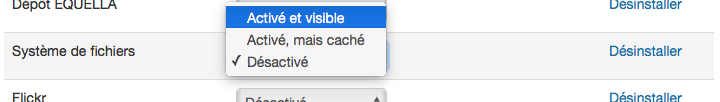
\includegraphics[width=10cm]{repo-filesystem-usb-1.png}
\end{minipage}
\end{figure}

On clique ensuite sur \emph{Enregistrer}, puis sur \emph{Paramètres} (même ligne), puis sur le bouton \emph{Créer une instance de dépôt}. Enfin, on sélectionne \emph{usb} dans le menu déroulant, et on indique \emph{USB Drive} dans le champ obligatoire \emph{Nom}.

\begin{figure}[!ht]
\begin{minipage}[b]{\linewidth}
\centering
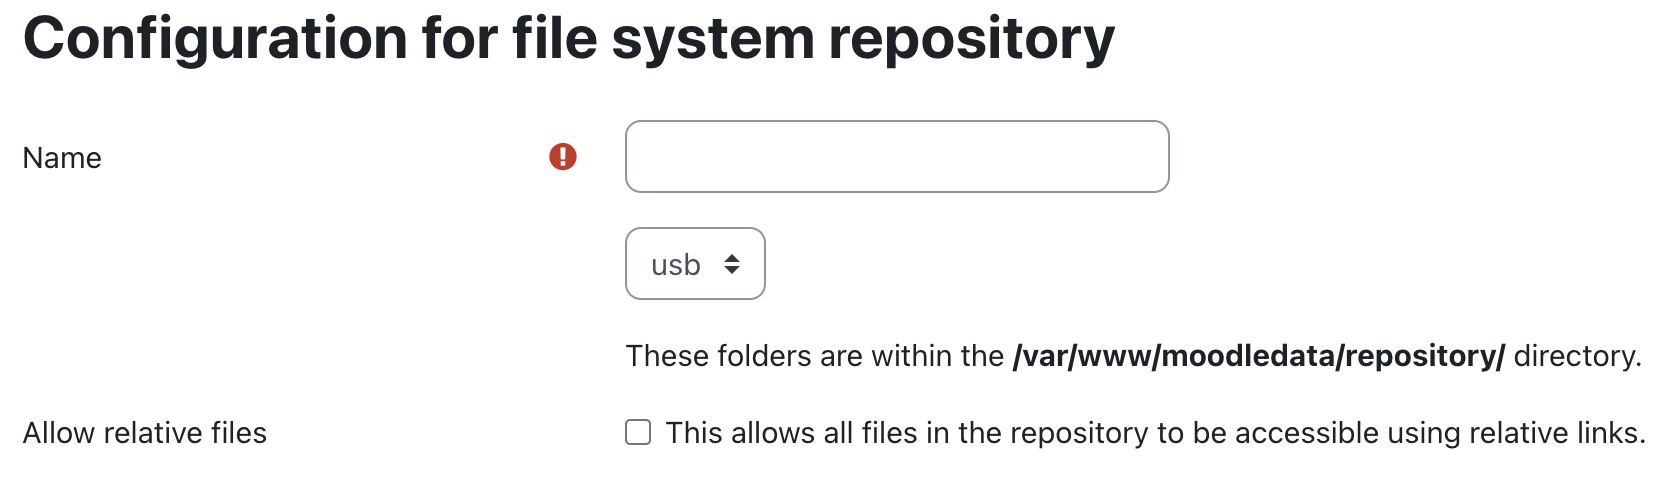
\includegraphics[width=11cm]{repo-filesystem-usb-2.png}
\end{minipage}
\end{figure}

\subsection{Fichiers déposés par SFTP}

On crée un dossier dans lequel les fichiers devront être déposés pour être accessibles depuis Moodle, ainsi qu'un lien vers le dossier de données de Moodle. Les permissions adéquates sont données.

\begin{lstlisting}[language=bash]
$ mkdir -p /home/moodlebox/files
$ sudo chown -R moodlebox:www-data files/
$ sudo chmod g+s files/
$ sudo ln -s /home/moodlebox/files /var/www/moodledata/repository
\end{lstlisting}

On effectue la configuration d'un dépôt \emph{Système de fichiers}, de façon similaire au dépôt « USB Drive » ci-dessus, en indiquant le dossier \emph{files} et en indiquant \emph{SFTP Documents} comme nom de dépôt.

Pour déposer des fichiers, on se connecte au moyen d'un logiciel SFTP\footnote{Par exemple : \href{https://filezilla-project.org/}{FileZilla}, \href{https://cyberduck.io/}{Cyberduck}, \href{http://winscp.net/}{WinSCP}.} sur la MoodleBox, avec le nom d'utilisateur \emph{moodlebox} et le mot de passe \emph{Moodlebox4\$}. Les fichiers seront déposés dans le dossier \lstinline{files}.

Installation de ghostscript et de poppler-utils

\section{Configurations additionnelles de Moodle}

\subsection{Activation de l'accès via l'app mobile de Moodle}

Après s'être connecté à la plateforme avec le compte administrateur,  on visite dans le Moodle \emph{Administration du site > Plugins > Services web > Mobile}. On coche la case \emph{Activer les services web pour appareils mobiles} et l'on enregistre les modifications.

Pour cette plateforme dont la destination n'est pas d'être publiée sur Internet, l'avertissement concernant le certificat SSL peut être ignoré sans risque.

\iffalse
\begin{verification}
Depuis un smartphone connecté en Wi-Fi sur le réseau MoodleBox, lancer l'app mobile Moodle et se connecter à la plateforme au moyen de l'URL \url{http://moodlebox.home}, avec le compte administrateur. Aucune erreur ne doit être signalée, et le message \emph{Aucune information de cours à afficher} est affiché sur l'écran du smartphone.
\end{verification}
\fi

\subsection{Installation du plugin Administration MoodleBox}

Afin de permettre le redémarrage et l'arrêt de la MoodleBox sans risque de corruption de la carte microSD, la modification du mot de passe, le réglage de l'heure, le changement du mot de passe du réseau Wi-Fi, ainsi que pour donner des informations utiles sur son fonctionnement, on installe le plugin d'administration \emph{MoodleBox} pour Moodle\footnote{Plugin MoodleBox \url{https://github.com/martignoni/moodlebox-plugin}.}.

Le plus simple est de l'installer au moyen de l'interface graphique de Moodle, en visitant \emph{Administration du site > Plugins > Dépôts > Installer des plugins}. On clique sur le bouton \emph{Installer des plugins à partir du répertoire des plugins Moodle} et choisit le plugin d'administration \emph{MoodleBox} (\emph{Admin tools}).

Il est aussi possible de l'installer via Git\footnote{Le code source du plugin MoodleBox est disponible à l'adresse \url{https://moodle.org/plugins/tool_moodlebox}.}.

\begin{lstlisting}[language=bash]
$ cd /var/www/moodle/admin/tool/
$ sudo git clone https://github.com/martignoni/moodlebox-plugin.git moodlebox
\end{lstlisting}

On termine dans ce cas l'installation du plugin en visitant la page \url{http://moodlebox.home/admin}. 

Pour finaliser l'installation du plugin, il est nécessaire de créer quelques fichiers et d'en régler les autorisations.
\begin{lstlisting}[language=bash]
$ cd /var/www/moodle/admin/tool/moodlebox
$ sudo touch .reboot-server; touch .shutdown-server; touch .set-server-datetime; touch .newpassword; touch .wifisettings
$ sudo chown -R www-data:moodlebox /var/www/moodle/admin/tool/moodlebox
$ sudo chmod -R ug+w,o-w /var/www/moodle/admin/tool/moodlebox
\end{lstlisting}

%:TODO: Replace incron with direvent
TODO: Replace incron with direvent

On installe finalement le paquetage \emph{incron}.

\begin{lstlisting}[language=bash]
$ sudo apt-get install -y incron
\end{lstlisting}

On autorise l'utilisation de \emph{incron} par \emph{root}, puis modifie la table des tâches de \emph{incron}.

\begin{lstlisting}[language=bash]
$ echo root | sudo tee -a /etc/incron.allow
$ sudo incrontab -e
\end{lstlisting}

en y ajoutant les lignes
\begin{lstlisting}[language=bash]
/var/www/moodle/admin/tool/moodlebox/.reboot-server IN_CLOSE_WRITE /sbin/shutdown -r now
/var/www/moodle/admin/tool/moodlebox/.shutdown-server IN_CLOSE_WRITE /sbin/shutdown -h now
/var/www/moodle/admin/tool/moodlebox/.set-server-datetime IN_MODIFY /bin/bash /var/www/moodle/admin/tool/moodlebox/.set-server-datetime
/var/www/moodle/admin/tool/moodlebox/.newpassword IN_CLOSE_WRITE /bin/bash /var/www/moodle/admin/tool/moodlebox/bin/changepassword.sh
/var/www/moodle/admin/tool/moodlebox/.wifisettings IN_CLOSE_WRITE /bin/bash /var/www/moodle/admin/tool/moodlebox/bin/changewifisettings.sh
\end{lstlisting}


\section{Configuration de Adminer}

\begin{lstlisting}[language=bash]
$ sudo apt-get install -y -t stretch phpmyadmin
$ sudo ln -s /usr/share/phpmyadmin /var/www/moodle/phpmyadmin
\end{lstlisting}
Définir un mot de passe fort. Pour cette installation, le mot de passe choisi est \emph{Moodlebox4\$}. Pour accéder à la totalité des fonctionnalités de PhpMyAdmin, on accèdera à l'interface au moyen de l'utilisateur \emph{moodlebox} et du mot de passe \emph{Moodlebox4\$}.

\iffalse
\begin{verification}
Charger l'URL \url{http://moodlebox.home/phpmyadmin/}. L'interface de PhpMyAdmin doit s'afficher. Pour s'y connecter, utiliser le nom d'utilisateur \emph{moodlebox} et le mot de passe \emph{Moodlebox4\$}.
\end{verification}
\fi

\section{Optimisation}

Pour que la MoodleBox soit utilisable en pratique, il est nécessaire de prendre soin à son optimisation. On configure ainsi le cache de Moodle, ainsi que sa gestion des dépôts et téléchargements de fichiers.

\subsubsection[Disque RAM pour certains dossiers de Moodle]{Disque RAM pour certains dossiers de Moodle\footnote{Cette section est en partie inspirée de \url{https://www.leading-interactive.de/e-learning/moodle-performance-tuning-mit-tmpfs/}.}}

Créer un dossier comme point de montage pour le disque RAM.
\begin{lstlisting}[language=bash]
$ sudo mkdir /var/cache/moodle
$ sudo chown www-data:moodlebox /var/cache/moodle/
$ sudo chmod ug+w,o-w /var/cache/moodle/
\end{lstlisting}

On utilise également des disques RAM pour le dossier temporaire et le dossiers des sessions de Moodle. Ces deux dossiers sont situés dans le dossier \emph{moodledata}.

On définit dans la table des partitions du Raspberry les disques RAM. Pour ce faire, on ajoute au fichier \lstinline{/etc/fstab}, les lignes suivantes
\begin{lstlisting}[language=bash]
tmpfs /var/cache/moodle tmpfs size=64M,mode=775,uid=www-data,gid=www-data 0 0
tmpfs /var/www/moodledata/temp tmpfs size=64M,mode=775,uid=www-data,gid=www-data 0 0
tmpfs /var/www/moodledata/sessions tmpfs size=32M,mode=775,uid=www-data,gid=www-data 0 0
\end{lstlisting}

%\begin{lstlisting}[language=bash]
%$ sudo nano /etc/fstab
%\end{lstlisting}
%
Le contenu du fichier \lstinline{/etc/fstab} sera alors :
\lstinputlisting[language=bash]{files/fstab}

Après un redémarrage de la Raspberry, le cache peut être configuré dans Moodle.

On se connecte à Moodle avec le compte administrateur (créé plus haut), puis dans le Moodle on visite \emph{Administration du site > Plugins > Cache > Configuration}. On crée deux nouvelles instances de dépôt, en cliquant sur \emph{Ajouter une instance} dans la section \emph{Entrepôts de cache installés} (en haut de la page).

\begin{figure}[!ht]
\begin{minipage}[b]{0.45\linewidth} % A minipage that covers half the page
\centering
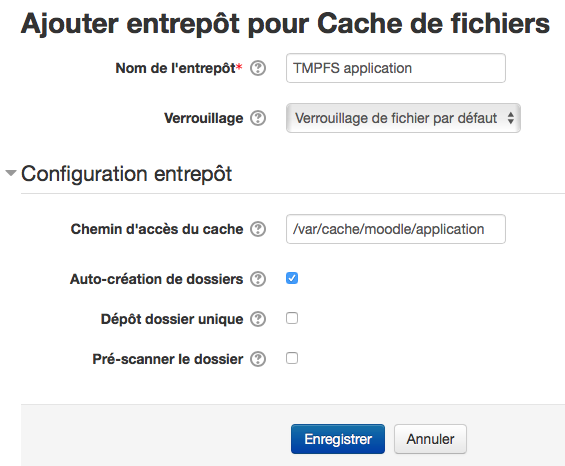
\includegraphics[width=7.3cm]{cache-application.png}
\end{minipage}
\hspace{\fill} % To get a little bit of space between the figures
\begin{minipage}[b]{0.45\linewidth}
\centering
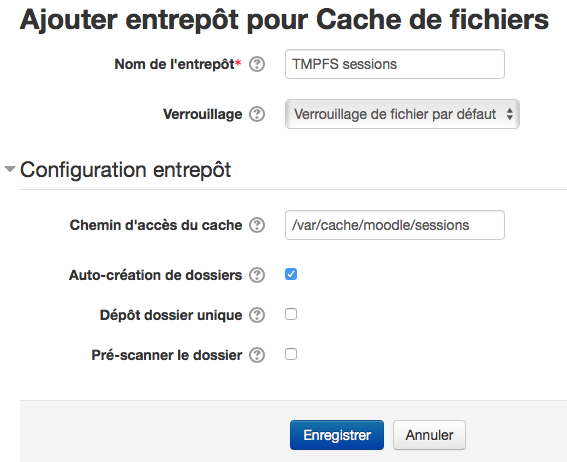
\includegraphics[width=7.3cm]{cache-sessions.png}
\end{minipage}
\end{figure}

\begin{enumerate}
\item Nom de l'entrepôt : \emph{TMPFS application}, chemin d'accès du cache : \emph{/var/cache/moodle/application}, cocher la case \emph{Auto-création de dossiers};
\item Nom de l'entrepôt : \emph{TMPFS sessions}, chemin d'accès du cache : \emph{/var/cache/moodle/sessions}, cocher la case \emph{Auto-création de dossiers}.
\end{enumerate}

Pour terminer, il reste à associer ces nouvelles instances de cache à leur destination, en cliquant sur \emph{Modifier les correspondances} tout en bas de la page, dans le domaine \emph{Entrepôts utilisés en l'absence de correspondance}.

\begin{figure}[!ht]
\begin{minipage}[b]{\linewidth}
\centering
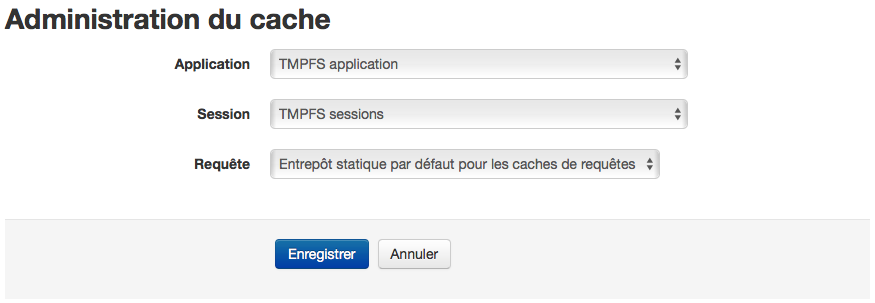
\includegraphics[width=11cm]{cache-association.png}
\end{minipage}
\end{figure}

\iffalse
\begin{verification}
Après quelques actions sur la plateforme Moodle de la MoodleBox, se connecter via SSH à la MoodleBox, puis lancer la commande
\begin{lstlisting}[language=bash]
ls -l /var/cache/moodle/
\end{lstlisting}
La console doit afficher quelque chose comme
\begin{lstlisting}[language=bash]
total 0
drwxrwxrwx 19 www-data www-data 380 mai   30 19:18 application
drwxrwxrwx  8 www-data www-data 160 mai   29 19:00 sessions
\end{lstlisting}
\end{verification}
\fi

Le cache en disque RAM a un défaut: les données qu'il contient disparaissent à chaque redémarrage de la MoodleBox. Moodle doit donc à chaque fois reconstruire le cache. Si l'on veut conserver le cache entre les redémarrages, on copie à intervalle régulier le contenu du disque RAM sur la carte microSD, et, lors de chaque démarrage, on effectue l'opération inverse.

On crée le dossier de sauvegarde, puis on définit le cron
\begin{lstlisting}[language=bash]
$ sudo mkdir /var/cache/moodle-cache-backup/
$ sudo crontab -e
\end{lstlisting}

On ajoute à la table des crons les deux lignes suivantes pour effectuer la sauvegarde du cache toutes les 20 minutes et pour restaurer le cache au démarrage:
\begin{lstlisting}[language=bash]
*/20 * * * * rsync -a --delete /var/cache/moodle/ /var/cache/moodle-cache-backup/
@reboot cp -Rpf /var/cache/moodle-cache-backup/* /var/cache/moodle/
\end{lstlisting}

\subsubsection{Optimisation de MariaDB}

On modifie les valeurs de quelques variables de MariaDB dans le fichier \lstinline{/etc/mysql/mariadb.conf.d/50-server.cnf}. Pour ce faire, on ouvre le fichier en question
et on y modifie les lignes adéquates, à savoir:
\begin{lstlisting}[language=bash]
table_cache             = 512
table_definition_cache  = 512
max_connections         = 100
query_cache_size        = 16M
query_cache_type        = 0
\end{lstlisting}

\section{Redimensionnement automatique de la partition}

Afin d'éviter à l'utilisateur de devoir redimensionner manuellement la partition de travail, on configure le redimensionnement automatique au premier démarrage. La méthode est identique à celle utilisée lors de la construction de l'image-disque de \emph{Raspbian Stretch Lite}\footnote{\url{https://github.com/RPi-Distro/pi-gen}}.

On copie le fichier \lstinline{resize2fs_once} ci-dessous dans le dossier \lstinline{/etc/init.d/}, et on lui donne les permissions adéquates pour être lancé au redémarrage.
\lstinputlisting[language=bash]{files/resize2fs_once}

Finalement, avant la dernière extinction précédant le clonage et le redimensionnement de l'image disque, on termine en lançant la commande
\begin{lstlisting}[language=bash]
$ sudo systemctl enable resize2fs_once
\end{lstlisting}
puis on ajoute à la fin de la ligne du fichier \lstinline{/boot/cmdline.txt} les instructions ci-dessous, immédiatement après le texte \lstinline{rootwait} (sans oublier un espace).
\begin{lstlisting}[language=bash]
quiet init=/usr/lib/raspi-config/init_resize.sh
\end{lstlisting}

Il est indispensable de ne pas redémarrer la MoodleBox, sans quoi l'opération décrite dans cette section devra être intégralement recommencée.

\section{Nettoyage de la distribution}

Les commandes ci-dessous permettent de nettoyer la MoodleBox et de diminuer l'espace disque qui lui est nécessaire, avant de la cloner et de la distribuer.

\begin{lstlisting}[language=bash]
$ sudo rm -r /var/www/moodledata/cache/*
$ sudo rm -r /var/www/moodledata/localcache/*
$ sudo rm -r /var/www/moodledata/temp/*
$ sudo rm -r /var/www/moodledata/trashdir/*
$ sudo rm -r /var/www/moodledata/sessions/*
$ sudo rm -r /var/cache/moodle/*
$ sudo rm -r /var/cache/moodle-cache-backup/*
$ sudo mysql moodle -e "truncate table moodle.mdl_logstore_standard_log"
$ sudo mysql moodle -e "truncate table moodle.mdl_config_log"
$ sudo mysql moodle -e "truncate table moodle.mdl_upgrade_log"
$ sudo apt-get clean
$ sudo rm -r /var/lib/apt/lists/*
$ sudo rm -r /var/cache/debconf/*
$ sudo rm -r /tmp/*
$ sudo rm -r /var/tmp/*
$ rm ~/.mysql_history
$ sudo bash -c 'for logs in `find /var/log -type f`; do > $logs; done'
$ cat /dev/null > ~/.bash_history && history -c && sudo shutdown -h now
\end{lstlisting}

Si tout s'est bien passé, la totalité a une taille d'environ 1.6~Go. L'image-disque, une fois tronquée, a une taille d'environ 1.9~Go. Compressée, elle tient dans environ 550~Mo.

\section{Acknowledgements}

MoodleBox utilise certaines idées de la première version de Christian Westphal\footnote{Christian Westphal, Académie de Strasbourg, voir \url{https://moodle.org/user/view.php?id=1378197&course=20}.}, qui mérite pour cela une gratitude particulière.

\end{document}
%%
%% The end
